% IF YOU ARE USING OVERLEAF, MAKE SURE TO SET THE COMPILER TO XeLaTeX
% (Menu in the top left > Settings > Compiler).

\documentclass[final]{beamer}

% ====================
% Packages
% ====================

\usepackage{standalone}
\usepackage{blochsphere}
\usepackage{ragged2e}
\usepackage{lipsum}
\usepackage{graphicx,epsfig}
\usepackage{amsmath,amsfonts,amssymb,amsthm}
\usepackage{array,tabularx,multirow,makecell,setspace}
\usepackage{comment}
\usepackage[T1]{fontenc}
\usepackage{lmodern}
\usepackage[size=custom,width=120,height=90,scale=1.0]{beamerposter}

%\usetheme{gemini}
\usetheme{avenirnext}
\usecolortheme{umbc}

\usepackage{booktabs}
\usepackage[svgnames]{xcolor}
\usepackage{caption}
\usepackage{subcaption}
\usepackage[labelfont={color=umbcaokteal}]{caption}
\usepackage{tikz}
\usetikzlibrary{calc,matrix,positioning,arrows.meta}
\usepackage{pgfplots}
\pgfplotsset{compat=1.17}

% ====================
% SUBMITTED ABSTRACT
% ====================

\begin{comment}
	Recent advances in quantum computing raise the question of whether quantum game-theoretic models produce different equilibrium outcomes than classical strategic games. One approach for exploring this question is quantum game theory, which extends classical game-theoretic models by incorporating concepts such as superposition and entanglement. In this framework, players’ strategies are represented by quantum operators acting on entangled states, allowing correlations that cannot arise in classical models and potentially affecting equilibrium outcomes. This work analyzed whether quantum game-theoretic models produced different equilibrium outcomes than classical frameworks. Two-player and multi-player versions of the Prisoner’s Dilemma and Chicken games were modeled in classical and quantum settings to evaluate differences in expected payoffs. Classical mixed and correlated equilibria were simulated in Python using payoff matrices and best-response dynamics to compute Nash equilibria. The quantum extension implemented the Eisert--Wilkens--Lewenstein quantization protocol in Qiskit to model entanglement and strategic operators. Preliminary results suggested that quantum correlations altered the payoff landscape and shifted equilibrium structures under certain parameter settings, while ongoing analysis examines stability across varying correlation strengths and scalability to multi-player systems.
\end{comment}

% ====================
% Lengths
% ====================

% If you have N columns, choose \sepwidth and \colwidth such that
% (N+1)\sepwidth + N\colwidth = \paperwidth
\newlength{\sepwidth}
\newlength{\colwidth}
\setlength{\sepwidth}{0.025\paperwidth}
\setlength{\colwidth}{0.3\paperwidth}

\newcommand{\separatorcolumn}{\begin{column}{\sepwidth}\end{column}}

% ====================
% Title Info
% ====================

\title{Equilibria in Classical and Quantum Strategic Games}

\author{
John Bui
\and Mohammadhossein Mohammadisiahroudi
\and Bed\v{r}ich Soused\'{i}k
}

\institute{
Department of Mathematics and Statistics, UMBC
}

% ====================
% Footer
% ====================

\footercontent{
  \href{https://johnlmbui.github.io/}{johnlmbui.github.io} \hfill
  Undergraduate Research and Creative Achievement Day (URCAD) 2026 \hfill
  \href{mailto:johnlmbui@umbc.edu}{johnlmbui@umbc.edu}
}

% ====================
% Body
% ====================

\begin{document}

\RaggedRight

% Top-right logo
\addtobeamertemplate{headline}{} {
    \begin{tikzpicture}[remember picture,overlay]
      \node[
        anchor=north east,
        inner sep=3.0cm
      ] at ([xshift=0.0cm,yshift=0.5cm]current page.north east)
      {
\includegraphics[height=3.5cm]{umbc_logos/UMBC-primary-logo-RGB.png}};
    \end{tikzpicture}
}

% Top-left QR code
\addtobeamertemplate{headline}{} {
	\begin{tikzpicture}[remember picture,overlay]
		\node[
		anchor=north west,
		inner sep=3.0cm
		] at ([xshift=0.0cm,yshift=2.3cm]current page.north west)
		{
\includegraphics[height=7cm]{qr-code.png}};
	\end{tikzpicture}
}

\begin{frame}[t]
\begin{columns}[t]
\separatorcolumn

% ====================
% Column 1
% ====================

\begin{column}{\colwidth}
	
	\begin{block}{Introduction}
		
		Bonnie and Clyde run an underground Elo boosting service in \textit{Riot of Retrievers}, the most popular MMORPG in the world. Business is booming, but as all good things must come to an end, they are eventually caught.
		
		Separated into solitary confinement with no communication, each must choose whether to \textbf{cooperate} (stay silent) or \textbf{defect} (snitch), leading to the following outcomes:
		
		\begin{table}
			\centering
			\caption{Possible scenarios from actions \{Cooperate, Defect\}.}
			\renewcommand{\arraystretch}{1.6}
			\begin{tabular}{
					@{}r
					>{\raggedright\arraybackslash}p{0.18\textwidth}
					>{\hspace{0.25em}\raggedright\arraybackslash}p{0.58\textwidth}
					@{}
				}
				\toprule
				& \textbf{Decision} & \textbf{Outcome} \\
				\midrule
				1. & Both cooperate &
				\textbf{Reward:} both banned for 1 month \\
				
				2. & \makecell[l]{One defects,\\ one cooperates} &
				\makecell[l]{\textbf{Temptation:} defector receives warning (no ban)\\
					\textbf{Sucker's payoff:} cooperator banned permanently} \\
				
				3. & Both defect &
				\textbf{Punishment:} both banned for 1 year \\
				\bottomrule
			\end{tabular}
		\end{table}
		
		Ban duration is inversely related to payoff. Define
		\[
		\text{Temptation } T = 3,\quad 
		\text{Reward } R = 2,\quad 
		\text{Punishment } P = 1,\quad 
		\text{Sucker's payoff } S = 0,
		\]
		so that $T > R > P > S$, yielding the following payoff matrix:
		\input{tikz/prisoners}
		
		Bonnie and Clyde both snitch on each other, resulting in a one-year ban each. If acting in self-interest is rational, why does it lead to a worse outcome than cooperation?
		
		\heading{This paradox is known as the prisoner's dilemma.}
		
	\end{block}
	
	
	\begin{block}{Background: Classical Game Theory}
		
		\textbf{Game theory} is the study of decision-making under \textit{interdependence}, where two or more players \textit{optimize} their own payoff while accounting for the actions of others\cite{doi:10.1142/10634}.
		
		\heading{How do we evaluate outcomes?}
		
		A strategy profile $s$ is:
		
		\begin{itemize}
			\item a \textbf{Nash equilibrium} if no player can improve their payoff by unilaterally changing their strategy:
			\[
			u_i(s_i, s_{-i}) \ge u_i(s_i', s_{-i})
			\]
			
			\item \textbf{Pareto efficient} if no alternative makes every player at least as well off and at least one strictly better off:
			\[
			u_i(s') \ge u_i(s) \ \text{for all } i,
			\qquad
			u_j(s') > u_j(s) \ \text{for some } j
			\]
		\end{itemize}
		
		\heading{The game of chicken}
		
		Chicken is another $2 \times 2$ symmetric, non-zero-sum game, similar to the prisoner's dilemma, but focused on avoiding mutual disaster. In \textbf{iterated play}, chicken and the prisoner's dilemma often lead to turn-taking\cite{doi:10.1177/1043463190002004004}\cite{Lau:2012aa} and sustained mutual cooperation\cite{Ikeda_2021}, respectively.
		
		\input{tikz/chicken}
		
		\begin{center}
			\textcolor{umbcred}{\textit{Can players like Bonnie and Clyde achieve mutual cooperation without communication?}}
		\end{center}
		
	\end{block}
	
\end{column}

\separatorcolumn

% ====================
% Column 2
% ====================

\begin{column}{\colwidth}
	
	\begin{block}{Background: Quantum Computing}
		
		\textbf{Quantum computing} processes information by exploiting phenomena from quantum mechanics: \textbf{superposition} and \textbf{entanglement}.
		
		\heading{Superposition}
		
		\begin{center}
			\begin{minipage}[t]{0.4\textwidth}
				\centering
				\begin{tikzpicture}
					\node at (0,3.2) {0};
					\fill[umbcaokteal] (1.2,3.2) circle (0.3);
					
					\node at (0,-3.2) {1};
					\fill[umbcred] (1.2,-3.2) circle (0.3);
				\end{tikzpicture}
				
				\captionof{figure}{A classical bit.}
			\end{minipage}
			\hfill
			\begin{minipage}[t]{0.4\textwidth}
				\centering
				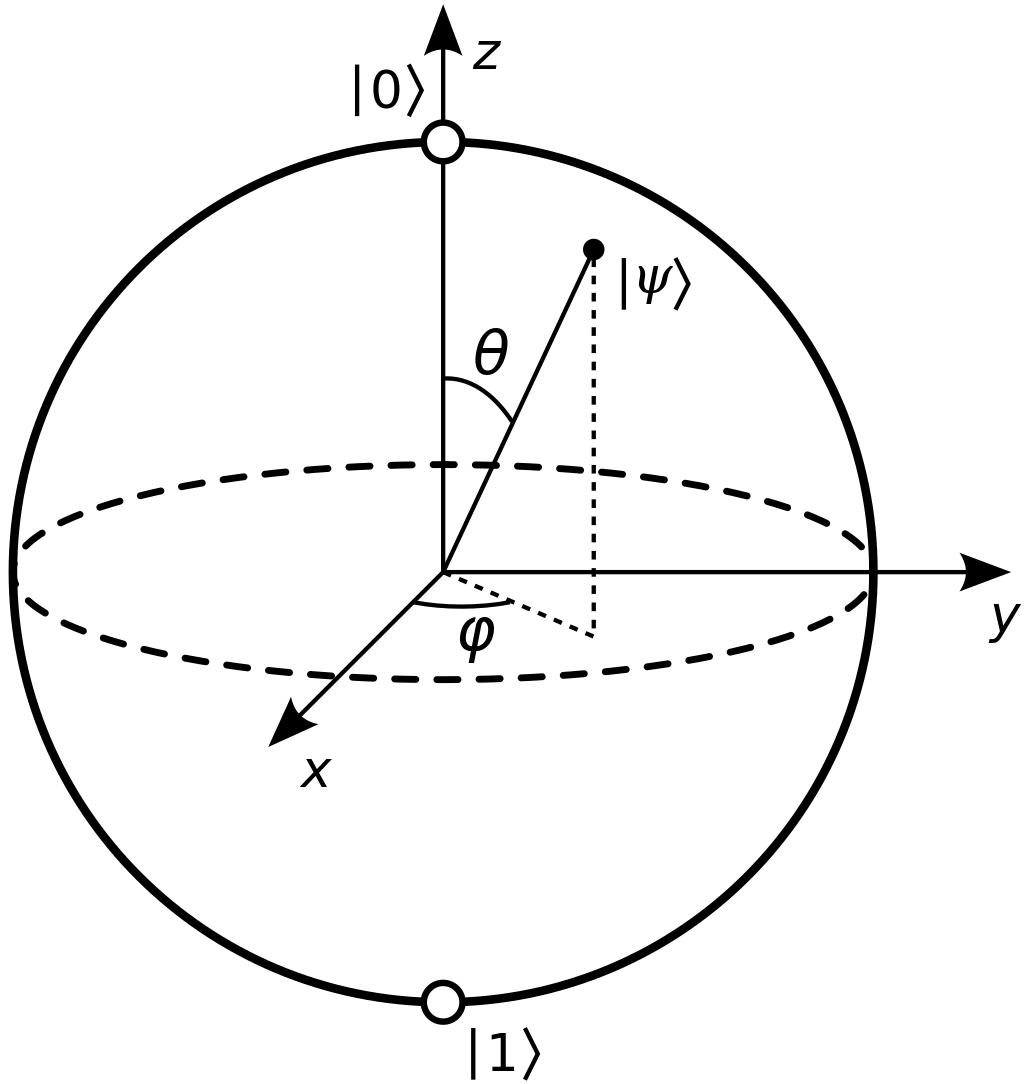
\includegraphics[width=0.7\linewidth]{bloch.png}
				
				\captionof{figure}{A qubit.}
			\end{minipage}
		\end{center}
		
		Classical bits store a single value ($0$ or $1$), while \textbf{qubits} exist in a \textbf{superposition} of states, representing multiple possibilities simultaneously:
		\[
		|\psi\rangle = \alpha |0\rangle + \beta |1\rangle, 
		\qquad
		|\alpha|^2 + |\beta|^2 = 1.
		\]
		
		\heading{Measurement problem}
		\textbf{Measurement} yields a single outcome with probabilities $|\alpha|^2$ and $|\beta|^2$.
		
		\begin{figure}
			\centering
			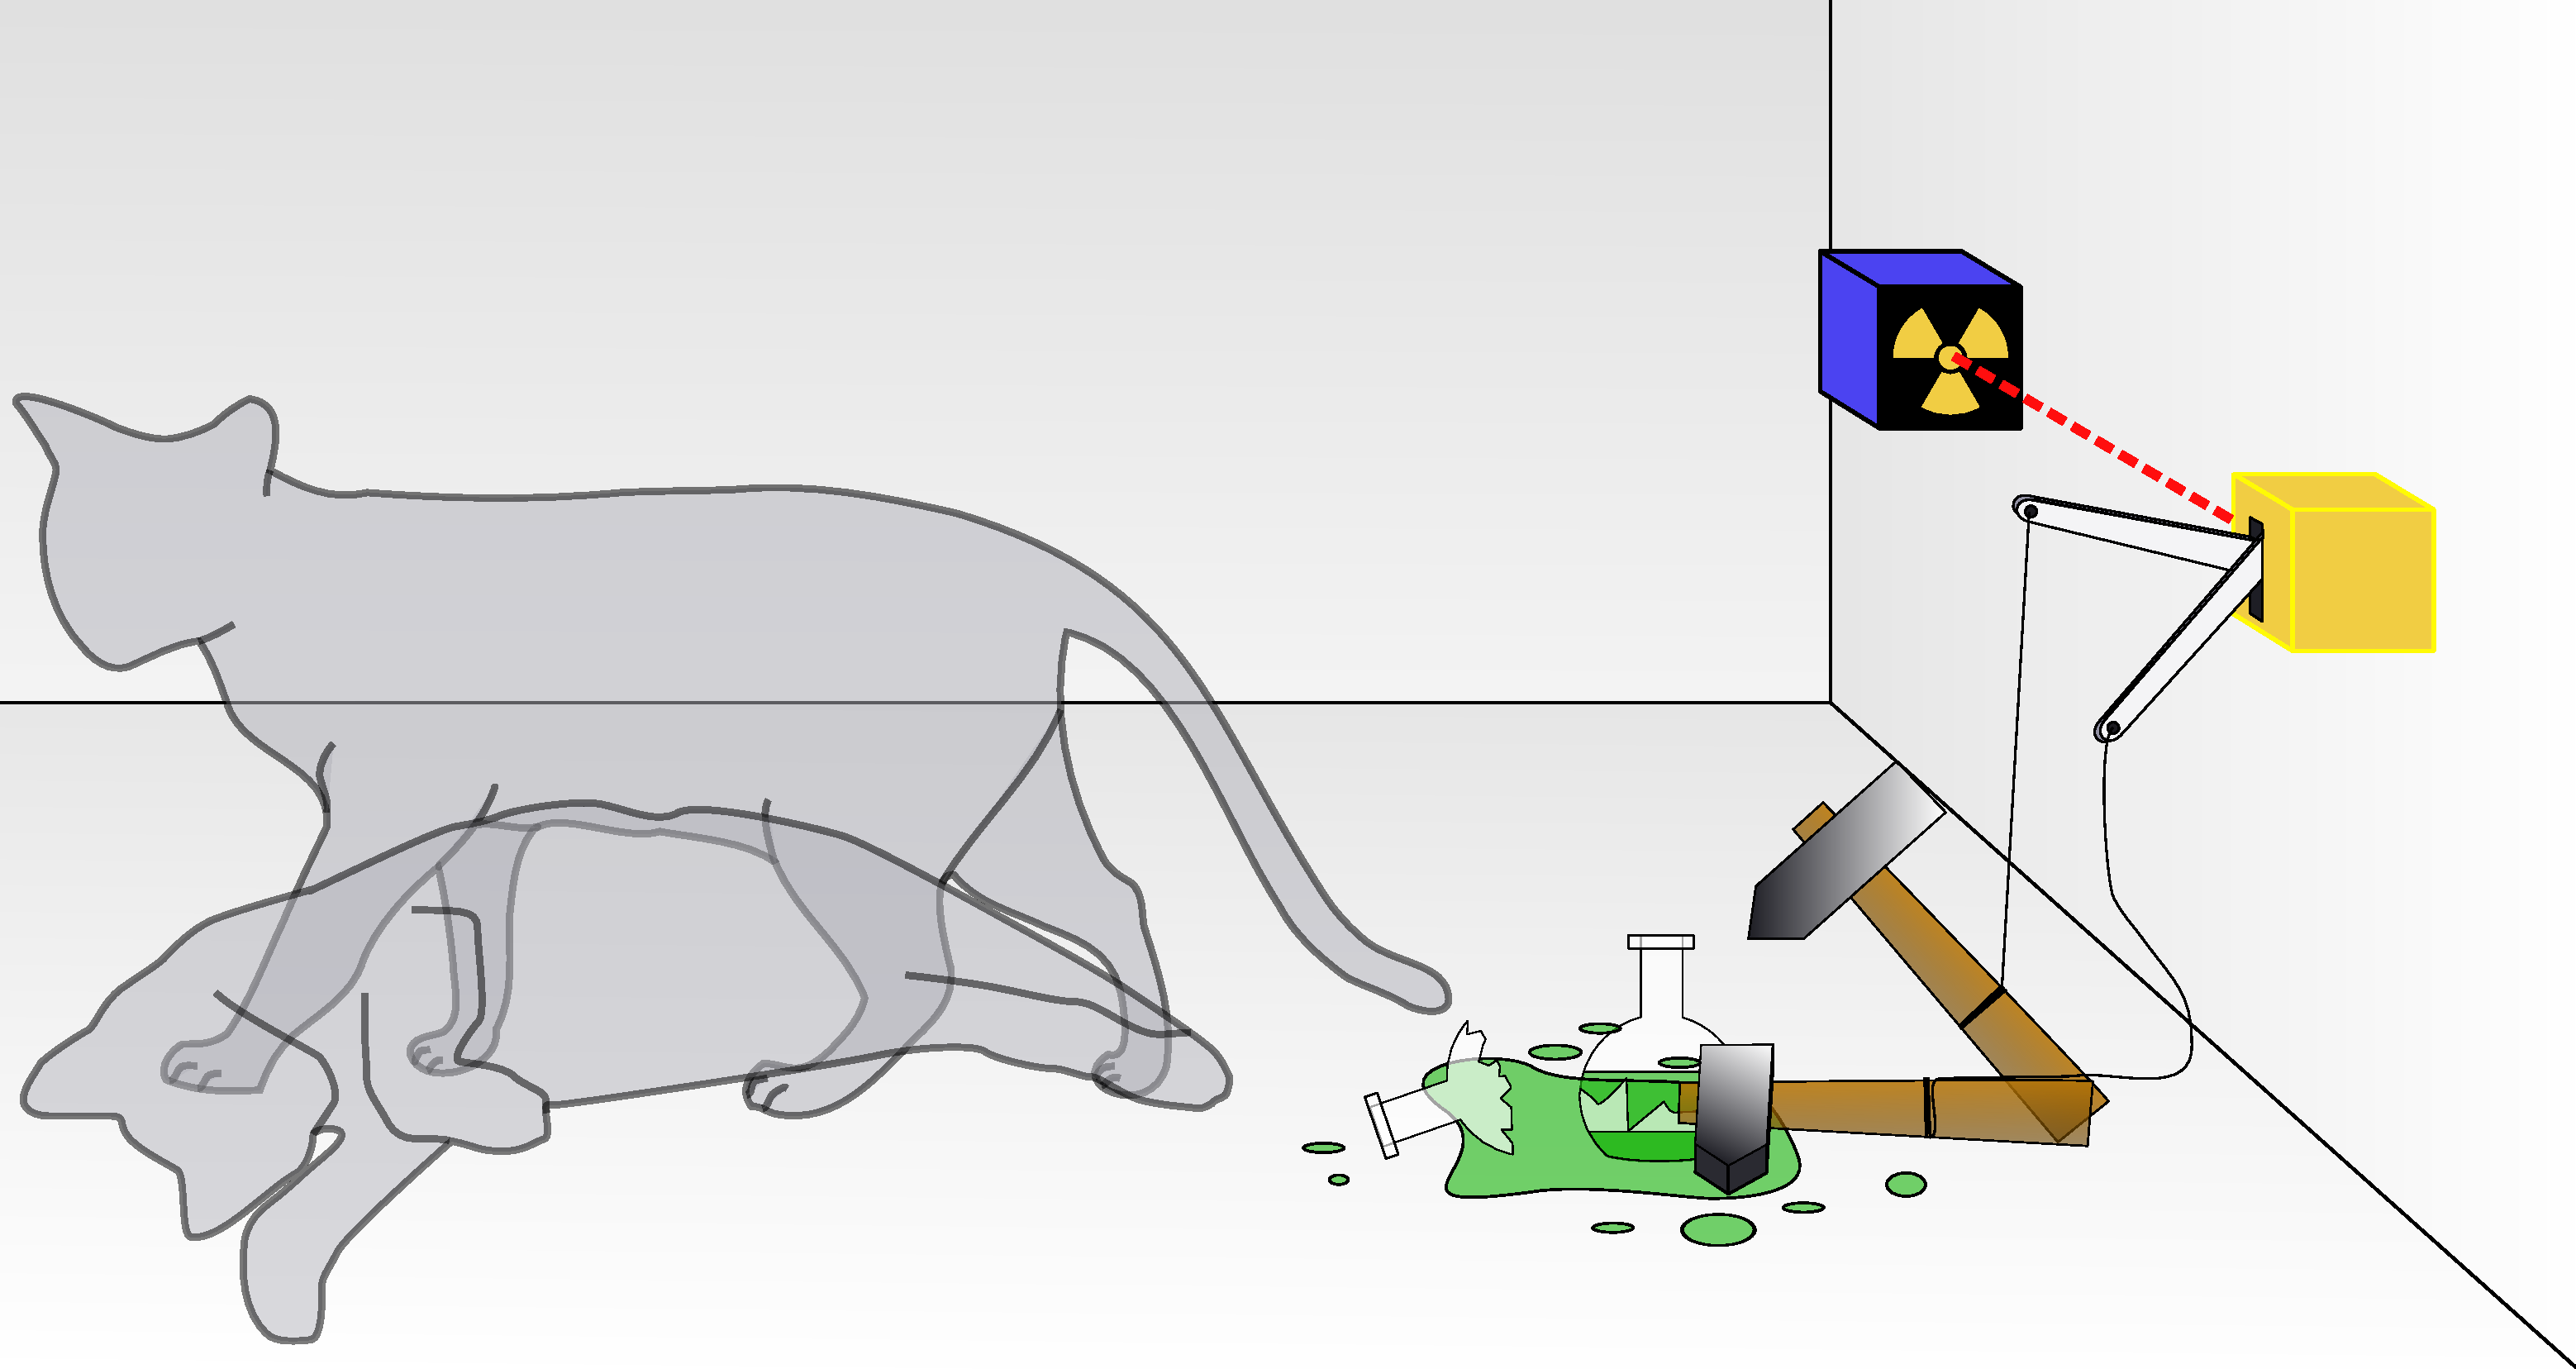
\includegraphics[width=0.4\textwidth]{Schrodingers_cat.pdf}
			\caption{Schr\"{o}dinger's cat (1935), illustrating quantum superposition before measurement.}
			\label{fig:cat}
		\end{figure}
		
		\heading{Entanglement}
		\textbf{Entangled systems} are linked, so measuring one reveals information about the other:
		\[
		|\psi\rangle \neq |\psi_A\rangle \otimes |\psi_B\rangle.
		\]
		
	\end{block}
	
	\begin{block}{Quantum Game Theory}
		
		Instead of choosing fixed actions (probability distributions), players apply \textbf{unitary transformations} to qubits, altering amplitudes that interfere to shape outcomes upon measurement.
		
		\heading{Quantum Prisoner's Dilemma}
		Eisert, Wilkens, and Lewenstein (1999) introduced a quantum version of the prisoner's dilemma, interpreting the basis states as strategies\cite{Eisert_1999}:
		\[
		|C\rangle = \text{Cooperate}, 
		\qquad 
		|D\rangle = \text{Defect}
		\]
		
		A general quantum strategy is a superposition of these states:
		\[
		|\psi\rangle = \alpha |C\rangle + \beta |D\rangle.
		\]
		
		Players act on qubits, producing outcomes in the joint state space:
		\[
		\{|CC\rangle, |CD\rangle, |DC\rangle, |DD\rangle\}.
		\]
		
		\begin{center}
			\captionof{table}{Joint quantum basis states for players' strategies.}
			\renewcommand{\arraystretch}{1.8}
			\resizebox{0.35\linewidth}{!}{%
				\begin{tabular}{c c c}
					& $|C\rangle_{P_2}$ & $|D\rangle_{P_2}$ \\
					
					\cline{2-3}
					$|C\rangle_{P_1}$ 
					& \multicolumn{1}{|c|}{$|CC\rangle$} 
					& \multicolumn{1}{c|}{$|CD\rangle$} \\
					
					\cline{2-3}
					$|D\rangle_{P_1}$ 
					& \multicolumn{1}{|c|}{$|DC\rangle$} 
					& \multicolumn{1}{c|}{$|DD\rangle$} \\
					
					\cline{2-3}
				\end{tabular}
			}
		\end{center}
		
		\end{block}
		
	\end{column}

\separatorcolumn

% ====================
% Column 3
% ====================

\begin{column}{\colwidth}
	
	\begin{block}{How Entanglement Changes the Game}
		
		Instead of randomizing over strategies, players manipulate amplitudes, with randomness arising only upon measurement. The game proceeds as follows:
		
		\heading{EWL Protocol}
		\begin{enumerate}
			\item Start in $|CC\rangle$.
			\item Apply the entangling operator $J$.
			\item Each player applies a local strategy $U_A \otimes U_B$.
			\item Apply $J^\dagger$ and measure, yielding
		\end{enumerate}
		
		\[
		|\psi_f\rangle = J^\dagger (U_A \otimes U_B) J |CC\rangle.
		\]
		
		\begin{center}
			\textit{The final state encodes all possible outcomes prior to measurement.}
		\end{center}
		
		\heading{Strategies and Payoffs}
		
		Players choose transformations $U(\theta,\phi)$ from a continuous set, representing a spectrum of quantum strategies, with classical strategies as special cases:
		\[
		C = I, \qquad
		D =
		\begin{pmatrix}
			0 & 1 \\
			-1 & 0
		\end{pmatrix}.
		\]
		
		Expected payoffs are computed from outcome probabilities:
		\[
		\mathbb{E}[u_A] = R P_{CC} + S P_{CD} + T P_{DC} + P P_{DD}.
		\]
		
		\heading{Entanglement and Correlation}
		
		Correlations between players influence outcomes, with $\gamma$ governing the transition from classical independence to quantum dependence:
		
		\[
		J = \exp\!\left(-i\frac{\gamma}{2}D \otimes D \right),
		\quad
		\gamma \in [0, \tfrac{\pi}{2}].
		\]
		
		\begin{center}
			\begin{tikzpicture}[scale=1.2]
				\draw[thick,->] (0,0) -- (10,0);
				
				\fill[umbcred] (0,0) circle (0.25);
				\fill[umbcaokteal] (5,0) circle (0.25);
				\fill[umbcgold] (10,0) circle (0.25);
				
				\node[below] at (0,-0.1) {$\gamma = 0$};
				\node[below] at (10,-0.1) {$\gamma = \frac{\pi}{2}$};
				
				\node[above,align=center] at (0,0.35)
				{\textbf{Classical}\\ $(D,D)$};
				
				\node[above,align=center] at (5,0.35)
				{\textbf{Transition}\\ correlations emerge};
				
				\node[above,align=center] at (10,0.35)
				{\textbf{Quantum}\\ $(Q,Q)$};
			\end{tikzpicture}
			\captionof{figure}{Increasing entanglement ($\gamma$) shifts the equilibrium from defection to cooperation.}
		\end{center}
		
		\heading{Key Result}
		
		Classically, $(D,D)$ is the unique Nash equilibrium but is Pareto inefficient. With maximal entanglement, this equilibrium disappears, and a new strategy emerges:
		\[
		Q =
		\begin{pmatrix}
			i & 0 \\
			0 & -i
		\end{pmatrix}.
		\]
		
		The profile $(Q,Q)$ is a Nash equilibrium with payoff $(R,R)$, making cooperation both stable (Nash equilibrium) and optimal (Pareto efficient).
		
		\textit{Conclusion.} Entanglement changes the \textbf{information structure} of the game, allowing players to coordinate without communication and escape the classical dilemma.
		
	\end{block}
	
	\begin{block}{Acknowledgments}
		
		I thank Mohammadhossein Mohammadisiahroudi and Bed\v{r}ich Soused\'{i}k for their mentorship and guidance, and Peter DeCrescenzo for his support through the UMBC Louis Stokes Alliance for Minority Participation (LSAMP). This work was supported, in part, by an Undergraduate Research Award from the UMBC Division of Undergraduate Academic Affairs.
		
	\end{block}
	
	
	\begin{block}{References}
		
		\nocite{*}
		\footnotesize{\bibliographystyle{plain}\bibliography{poster}}
		
	\end{block}
	
\end{column}

\separatorcolumn
\end{columns}
\end{frame}

\end{document}